\documentclass{beamer}

\mode<presentation> {
\usetheme{Rochester}
%\setbeamertemplate{footline} % To remove the footer line in all slides uncomment this line
%\setbeamertemplate{footline}[page number] % To replace the footer line in all slides with a simple slide count uncomment this line
\setbeamertemplate{footline}
{
  \leavevmode%
  \hbox{%
  \begin{beamercolorbox}[wd=\paperwidth,ht=2.25ex,dp=1ex,right]{title in head/foot}%
    \insertframenumber{} / \inserttotalframenumber\hspace*{1ex}
  \end{beamercolorbox}}%
  \vskip0pt%
}
\setbeamertemplate{navigation symbols}{} % To remove the navigation symbols from the bottom of all slides uncomment this line
}

\usepackage{graphicx} % Allows including images
\usepackage{booktabs} % Allows the use of \toprule, \midrule and \bottomrule in tables
\usepackage{multirow}
\usepackage{caption}
\usepackage{subfigure}
\usepackage{advdate}
\usepackage[lined,ruled,vlined,linesnumbered]{algorithm2e}

% Setup TikZ

\usepackage{tikz}
\usetikzlibrary{shapes,arrows}
\usetikzlibrary{positioning}
\tikzstyle{block}=[draw opacity=0.7,line width=1.4cm]
\tikzstyle{decision} = [diamond, draw, fill=blue!20, text width=4.5em, text badly centered, node distance=3cm, inner sep=0pt]
\tikzstyle{block} = [rectangle, draw, fill=blue!20, text width=5em, text centered, rounded corners, minimum height=4em]
\tikzstyle{implementation} = [rectangle, draw, fill=black!80, text width=5em, text centered, rounded corners, minimum height=4em]
\tikzstyle{specification} = [rectangle, draw, fill=white!20, text width=5em, text centered, rounded corners, minimum height=4em]
%\tikzstyle{line} = [draw, -latex']
\tikzstyle{line} = [draw]
\tikzstyle{cloud} = [draw, ellipse,fill=red!20, node distance=3cm, minimum height=2em]
\tikzset{onslide/.code args={<#1>#2}{%
  \only<#1>{\pgfkeysalso{#2}} % \pgfkeysalso doesn't change the path
}}

\usetikzlibrary{decorations.pathmorphing}
\tikzset{snake it/.style={decorate, decoration=snake}}

\tikzset{
    invisible/.style={opacity=0,text opacity=0},
    visible on/.style={alt={#1{}{invisible}}},
    alt/.code args={<#1>#2#3}{%
      \alt<#1>{\pgfkeysalso{#2}}{\pgfkeysalso{#3}} % \pgfkeysalso doesn't change the path
    },
}


\SetKwFor{ForEachP}{foreach}{in parallel do}{end}

%----------------------------------------------------------------------------------------
%	TITLE PAGE
%----------------------------------------------------------------------------------------

\title{Algorithmic Optimization and Parallelization
of Eppstein's Synchronizing Heuristic} 

\author[S. Karahoda]{Serta\c{c} Karahoda}
\institute[Sabanc\i{} Univ.] % Your institution as it will appear on the bottom of every slide, may be shorthand to save space
{Computer Science and Engineering, Faculty of Science and Engineering, Sabanc\i{} University, Tuzla, \.{I}stanbul, Turkey
}
\date{\DayAfter[1]} % Date, can be changed to a custom date


\begin{document}

\begin{frame}
\titlepage % Print the title page as the first slide
\end{frame}

\begin{frame}
\frametitle{Overview} % Table of contents slide, comment this block out to remove it
\tableofcontents 
\end{frame}

%----------------------------------------------------------------------------------------
%	PRESENTATION SLIDES
%----------------------------------------------------------------------------------------

%------------------------------------------------
\section{Preliminaries}

\begin{frame}{What is an Automaton?}
\begin{center}
	\scalebox{0.9}{
		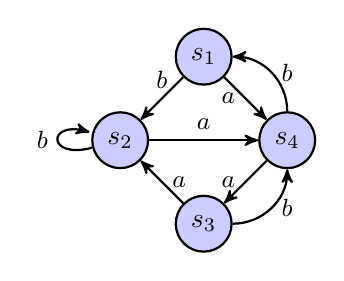
\begin{tikzpicture}[->,>=stealth',auto,node distance=15mm, thick,main node/.style={circle,fill=blue!20,draw}]
		
		\node[main node] (1) {$s_1$};
		\node[main node] (2) [below left of=1] {$s_2$};
		\node[main node] (3) [below right of=2] {$s_3$};
		\node[main node] (4) [below right of=1] {$s_4$};
		
		\path[every node/.style={font=\sffamily\small}]
		(1) edge node [left] {$a$} (4)
		edge node [above] {$b$} (2)
		(2) edge node {$a$} (4)
		edge [loop left] node {$b$} (2)
		(3) edge node [right] {$a$} (2)
		edge [out=0,in=-90] node[right] {$b$} (4)
		(4) edge node [left] {$a$} (3)
		edge [out=90,in=0] node[right] {$b$} (1);
		\end{tikzpicture}}
	\end{center}
	\vspace*{-2mm}
	\begin{block}{Definition}
		A \alert{deterministic and complete finite automaton $\cal A$} is defined by a triple ${\cal A}=(S,\Sigma,\delta)$.
		\begin{itemize}
			\item $S = \{ s_1, s_2, \ldots, s_n \}$: a finite set of states 
			\item $\Sigma = \{ x_1, x_2, \ldots, x_k \}$: A finite set of input symbols 
			\item $\delta : S \times \Sigma \rightarrow S$: A transition function which is \alert{total}
		\end{itemize}
	\end{block}
\end{frame}

\begin{frame}{Applying a Word to a State}
	\begin{block}{Definition}
		A \alert{word} or \alert{input sequence} $w$ is a sequence of input symbols (i.e. $w \in \Sigma^{\star}$). For example, {\color{blue}{$bbabaa$}} is a word.
	\end{block}
\vspace*{-2mm}

	\begin{center}
		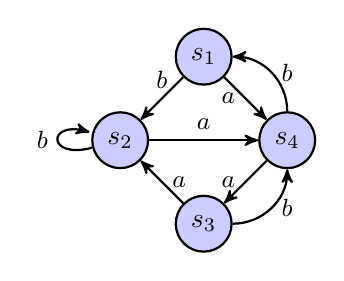
\begin{tikzpicture}[->,>=stealth',auto,node distance=15mm, thick,main node/.style={circle,fill=blue!20,draw}]
		
		\node[main node] (1) {$s_1$};
		\node[main node] (2) [below left of=1] {$s_2$};
		\node[main node] (3) [below right of=2] {$s_3$};
		\node[main node] (4) [below right of=1] {$s_4$};
		
		\path[every node/.style={font=\sffamily\small}]
		(1) edge node [left] {$a$} (4)
		edge node [above] {$b$} (2)
		(2) edge node {$a$} (4)
		edge [loop left] node {$b$} (2)
		(3) edge node [right] {$a$} (2)
		edge [out=0,in=-90] node[right] {$b$} (4)
		(4) edge node [left] {$a$} (3)
		edge [out=90,in=0] node[right] {$b$} (1);
		\end{tikzpicture}
	\end{center}
\vspace*{-2mm}
	
	\begin{block}{Definition}
		When \alert{a sequence $w$ is applied to a state $s_i$}, we take the walk that starts
		from $s_i$ with the path labeled by $w$. For example, $\delta(s_1,{\color{blue}abb}) = s_2$.
	\end{block}
\end{frame}

\begin{frame}{Applying an Input Sequence to a Set of States}
	\begin{center}
	\scalebox{0.9}{
		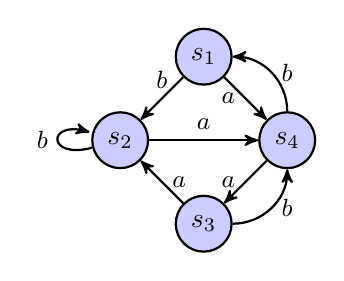
\begin{tikzpicture}[->,>=stealth',auto,node distance=15mm, thick,main node/.style={circle,fill=blue!20,draw}]
		
		\node[main node] (1) {$s_1$};
		\node[main node] (2) [below left of=1] {$s_2$};
		\node[main node] (3) [below right of=2] {$s_3$};
		\node[main node] (4) [below right of=1] {$s_4$};
		
		\path[every node/.style={font=\sffamily\small}]
		(1) edge node [left] {$a$} (4)
		edge node [above] {$b$} (2)
		(2) edge node {$a$} (4)
		edge [loop left] node {$b$} (2)
		(3) edge node [right] {$a$} (2)
		edge [out=0,in=-90] node[right] {$b$} (4)
		(4) edge node [left] {$a$} (3)
		edge [out=90,in=0] node[right] {$b$} (1);
		\end{tikzpicture}}
	\end{center}	
\vspace*{-2mm}
	\begin{block}{Definition}
		\begin{itemize}
			\item When \alert{a word $w$ is applied to \underline{a set of states} $C \subseteq S$}, 
			we consider all the walks that start from the states $s_i \in C$ with the path 
			labeled by $w$.\\
			For example, $\delta(\{s_1,s_2,s_4\},{\color{blue}abb}) = \{ s_1, s_2\}$.
			\item For any $C \subseteq S$ and for any $w \in \Sigma^{\star}$: $|\delta(C,w)| \leq |C|$\\
			($\cal A$ is deterministic \& states may merge).
		\end{itemize}
	\end{block}
	
\end{frame}

\begin{frame}{Definition of a Merging Sequence}
	\begin{center}
		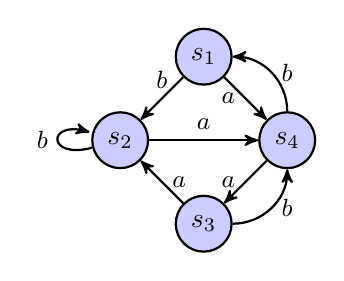
\begin{tikzpicture}[->,>=stealth',auto,node distance=15mm, thick,main node/.style={circle,fill=blue!20,draw}]
		
		\node[main node] (1) {$s_1$};
		\node[main node] (2) [below left of=1] {$s_2$};
		\node[main node] (3) [below right of=2] {$s_3$};
		\node[main node] (4) [below right of=1] {$s_4$};
		
		\path[every node/.style={font=\sffamily\small}]
		(1) edge node [left] {$a$} (4)
		edge node [above] {$b$} (2)
		(2) edge node {$a$} (4)
		edge [loop left] node {$b$} (2)
		(3) edge node [right] {$a$} (2)
		edge [out=0,in=-90] node[right] {$b$} (4)
		(4) edge node [left] {$a$} (3)
		edge [out=90,in=0] node[right] {$b$} (1);
		\end{tikzpicture}
	\end{center}
	\begin{block}{Definition}
		Let ${\cal A}=(S, \Sigma, \delta)$, a sequence $w$ is a \alert{merging sequence for $C \subseteq S$} if
		$\delta(C,r)$ is singleton. If $C=S$\ then the sequence $w$ is a \alert{reset word for $\cal A$}\
		For example:\\
		$\bullet$ {\color{blue}$b$} is merging sequence for {\color{blue}$\{s_1,s_2\}$}\\
		$\bullet$ {\color{blue}$bbb$} is merging sequence for {\color{blue}$\{s_1,s_3\}$} (it is in fact a reset word)
	\end{block}
\end{frame}

\begin{frame}{Do all automata have a reset word?}
	An automaton $\cal A$ is called \alert{synchronizing} or \alert{synchronizable} if there exists a reset word of it.

\underline{Not all automata has a reset word!}

Luckily, it is quite easy to check whether an automaton is synchronizable or not.
\end{frame}

\begin{frame}{Definition of a Pair Automaton}
	\begin{block}{Definition}
	An automaton which is produced from the set of pairs $S^{\langle 2 \rangle}$; ${\cal A}^{\langle 2 \rangle}=(S^{\langle 2 \rangle},\Sigma,\delta^{\langle 2 \rangle})$ is called a \textit{pair automaton}.
		\begin{itemize}
			\item $S^{\langle 2 \rangle} = \{ \{s_1, s_1 \}, \{s_1, s_2 \},  \ldots, \{s_n, s_n \} \}$: a set of multisets with length $\leq 2$
			\item $\delta^{\langle 2 \rangle} : S^{\langle 2 \rangle} \times \Sigma \rightarrow S^{\langle 2 \rangle}$: the transition function for the generated pair automaton.
		\end{itemize}
	\end{block}
\end{frame}

\begin{frame}{Checking Synchronizablity}

	\begin{block}{Proposition}
		An automaton ${\cal A}=(S,\Sigma,\delta)$ is synchronizing iff $\forall s_i,s_j \in S$, there exists a merging sequence for $\{ s_i, s_j \}$ i.e., An automaton $\cal A$ is synchronizable iff singletons are reachable from every pairs in ${\cal A}^{\langle 2 \rangle}$. 
	\end{block}
	
	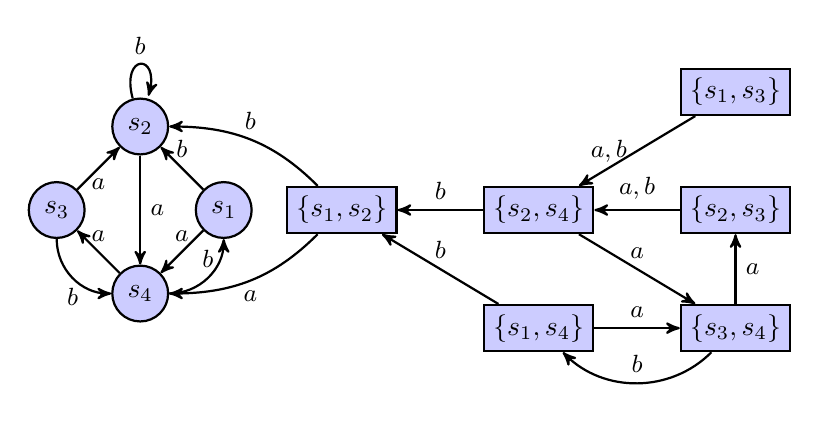
\begin{tikzpicture}[->,>=stealth',auto,node distance=15mm, thick,main node/.style={circle,fill=blue!20,draw},pair node/.style={rectangle,fill=blue!20,draw}]
		\node[main node] (2) {$s_2$};
		\node[main node] (3) [below left of=2] {$s_3$};
		\node[main node] (4) [below right of=3] {$s_4$};
		\node[main node] (1) [below right of=2] {$s_1$};
		\node[pair node] (1_2) [right of=1] {$\{ s_1, s_2 \}$};
		\node[pair node] (2_4) [right of=1_2, xshift=10mm] {$\{ s_2, s_4 \}$};
		\node[pair node] (1_4) [below of=2_4] {$\{ s_1, s_4 \}$};
		\node[pair node] (2_3) [right of=2_4, xshift=10mm] {$\{ s_2, s_3 \}$};
		\node[pair node] (1_3) [above of=2_3] {$\{ s_1, s_3 \}$};
		\node[pair node] (3_4) [below of=2_3] {$\{ s_3, s_4 \}$};
				
		
		\path[every node/.style={font=\sffamily\small}]
			(1) edge node [above] {$a$} (4)
				edge node [above] {$b$} (2)
			(2) edge node {$a$} (4)
				edge [loop above] node {$b$} (2)
			(3) edge node [below] {$a$} (2)
				edge [out=-90,in=180] node[below] {$b$} (4)
			(4) edge node [above] {$a$} (3)
				edge [out=0,in=-90] node[above] {$b$} (1)
			(1_2) edge [in=0, out=-135] node [below] {$a$} (4)
			 	  edge [in=0, out=135] node [above] {$b$} (2)
			(2_4) edge node [above] {$a$} (3_4)
				edge node [above] {$b$} (1_2)
			(1_3) edge node [left] {$a,b$} (2_4)
			(1_4) edge node [above] {$a$} (3_4)
				edge node [above] {$b$} (1_2)
			(2_3) edge node [above] {$a,b$} (2_4)
			(3_4) edge node [right] {$a$} (2_3)
				edge [in=-45, out=-135] node [above] {$b$} (1_4);
			 
	\end{tikzpicture}
\end{frame}



\section{Eppstein's Algorithm}

\begin{frame}{Synchronizing Heuristics}
	\begin{figure}
		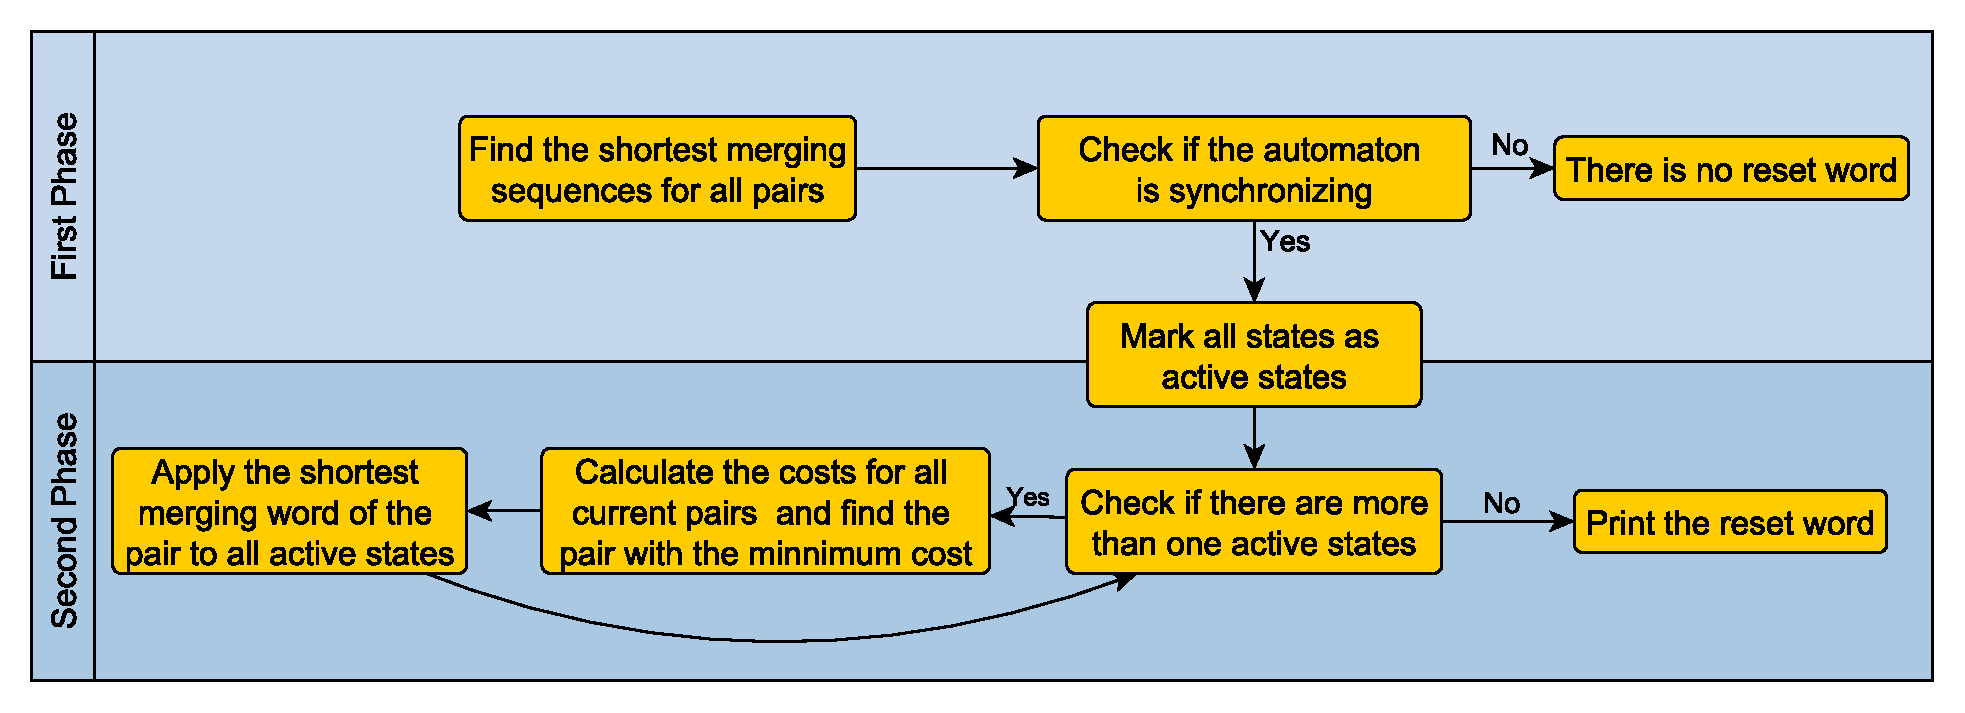
\includegraphics[width=\textwidth]{figs/heuristic_flow.pdf}
	\end{figure}
\end{frame}

\begin{frame}{\textsc{Greedy} Algorithm}
	\begin{itemize}
		\item One of the fastest synchronizing heuristics
		\item The cost of a pair: the length of the merging sequence
	\end{itemize}
\end{frame}
%
%\begin{frame}{\textsc{Greedy} Algorithm}
%	\small
%	\begin{algorithm}[H]
%	\caption{Eppstein's \textsc{Greedy} Algorithm}
%	\label{algo:greedy}
%	
%	\SetKwInOut{Input}{input}\SetKwInOut{Output}{output}
%	\Input{An automaton ${\cal A}=(S,\Sigma,\delta)$}
%	\Output{A reset word $\Gamma$ for ${\cal A}$ (or fail if ${\cal A}$ is not synchronizable)}
%	
%	%{--- Phase 1 ---}
%	compute a pairwise merging function (PMF) $\tau$\;
%	\If{there exists a pair $\{ s_i,s_j \}$ such that  $\tau(\{ s_i,s_j \})$ is undefined}
%	{
%		report that ${\cal A}$ is not synchronizable and exit;	
%	}
%
%	
%	%{--- Phase 2 ---}
%	$C = S$; \tcp{$C$ will keep track of the current set of states}
%	$\Gamma = \varepsilon$; \tcp{$\Gamma$ is the synchronizing sequence to be constructed}
%	
%	\While(\tcp*[h]{two or more states yet to be merged}){$|C| > 1$}
%	{
%		$\{ s_i,s_j \} = Find\_Min(C, \tau)$\;
%		
%		
%		$\Gamma = \Gamma \; \tau(\{ s_i,s_j \})$\;
%		$C = \delta(C,\tau(\{ s_i,s_j \}))$;
%	}
%	\end{algorithm}
%\end{frame}

\begin{frame}{Analysis on \textsc{Greedy}}
	\begin{table}[ht]
		\scalebox{0.7}{
			\begin{tabular}{r|rrr|rrr|rrr}
				&\multicolumn{3}{|c}{$n = 2000$}&\multicolumn{3}{|c}{$n = 4000$}&\multicolumn{3}{|c}{$n = 8000$}\\
				$p$ & $t_{PMF}$ & $t_{ALL}$ & $\frac{t_{PMF}}{t_{ALL}}$ & $t_{PMF}$ & $t_{ALL}$ & $\frac{t_{PMF}}{t_{ALL}}$ & $t_{PMF}$ & $t_{ALL}$ & $\frac{t_{PMF}}{t_{ALL}}$\\\hline
				2		& 0.172	& 0.185	& 0.929	& 1.184		& 1.240		& 0.954	& 5.899		& 6.325		& 0.933 \\
				8		& 0.504	& 0.517	& 0.975	& 2.709		& 2.768		& 0.978	& 14.289	& 14.721	& 0.971 \\
				32		& 2.113	& 2.126	& 0.994	& 9.925		& 9.986		& 0.994	& 51.783	& 52.233	& 0.991 \\
				128		& 9.126	& 9.140	& 0.999	& 40.356	& 40.418	& 0.998	& 193.548	& 193.982	& 0.998 \\
				\v{C}ern\'y	& 0.096	& 4.836	& 0.020	& 1.026		& 42.771	& 0.024	& 5.584		& 797.692	& 0.007
			\end{tabular}
		}
		\caption{Sequential PMF construction time ($t_{PMF}$), i.e., the first phase, and overall time ($t_{ALL}$) in seconds}
		\label{table:phase-comparison}
	\end{table}
\end{frame}

\begin{frame}{Analysis on \textsc{Greedy}}
\begin{table}[ht]
	\center
	\scalebox{0.7}{
	\begin{tabular}{r|rrr|rrr|rrr}
 		& \multicolumn{3}{c|}{n=2000} & \multicolumn{3}{c|}{n=4000} & \multicolumn{3}{c}{n=8000} \\
		p &  $h_{PMF}$ &  $h_{max}$ &  $h_{mean}$ &  $h_{PMF}$ &  $h_{max}$ &  $h_{mean}$ &  $h_{PMF}$ &  $h_{max}$ &  $h_{mean}$ \\ \hline
 		2 &  14.2 &  10.0 &  1.9 &  15.5 &  11.2 &  1.9 &  16.9 &  12.1 &  1.9 \\
 		8 &  5.0 &  4.0 &  1.3 &  6.0 &  4.2 &  1.3 &  6.0 &  4.6 &  1.3 \\
		32 &  3.1 &  2.7 &  1.1 &  4.0 &  2.9 &  1.1 &  4.0 &  3.0 &  1.1 \\
		128 &  3.0 &  2.0 &  1.0 &  3.0 &  2.0 &  1.0 &  3.0 &  2.1 &  1.0 \\
%		\v{C}ern\'y & 1999000.0 & 1952000.0 & 8884.8 & 7998000.0 & 7808000.0 & 19750.8 & 31996000.0 & 31232000.0 & 43480.8
	\end{tabular}}
	\caption{The length of longest merging sequence in PMF($h_{PMF}$) constructed in the first phase for random automata; maximum ($h_{max}$), and average ($h_{mean}$) lengths for merging sequences, used in the second phase of \textsc{Greedy}.}
\end{table}
\end{frame}

\begin{frame}{How can we make \textsc{Greedy} faster?}
	\textbf{Problem:}	
	\begin{itemize}
		\item  The execution time of the first phase dominates the overall execution time yet there is an exception (\v{C}ern\'y automata).
		\item The second phase does not need fully constructed PMF.
	\end{itemize}
	\textbf{Solution:}
	\begin{itemize}
		\item Parallelization of the first phase
		\item Parallelization of the second phase for slowly synchronizing automata
		\item Lazy computation for the first phase
	\end{itemize}
\end{frame}


\begin{frame}{The First Phase}

	\begin{figure}
		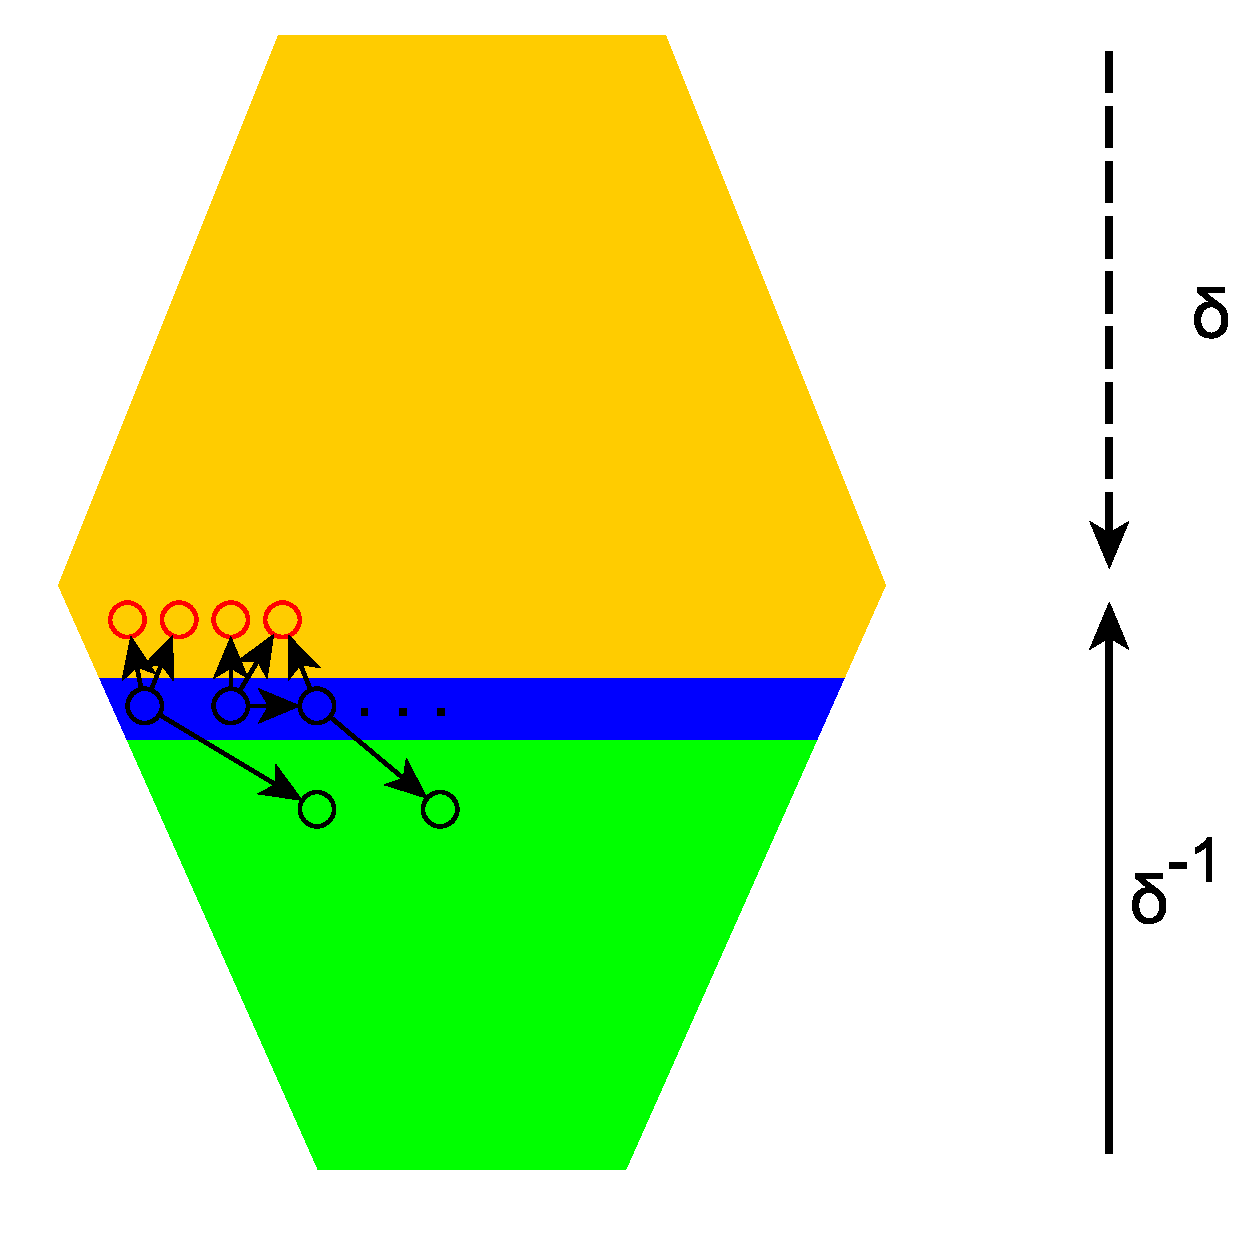
\includegraphics[height=0.8\textheight]{figs/f2r.pdf}
		%\caption{The figure summarizes the PMF construction phase.}
	\end{figure}
\end{frame}
%
%\begin{frame}{The First Phase}
%\begin{algorithm}[H]
%	\caption{Computing a PMF $\tau : S^{\langle 2 \rangle} \rightarrow \Sigma^\star$}
%	\label{algo:BFS}
%	\SetKwInOut{Input}{input}\SetKwInOut{Output}{output}
%	\Input{An automaton ${\cal A}=(S,\Sigma,\delta)$}
%	\Output{A PMF $\tau : S^{\langle 2 \rangle} \rightarrow \Sigma^\star$}
%	
%	%compute the reverse automaton ${A}^{-1} = (S,\Sigma,\delta^{-1})$ of $A$\;
%	\lForEach{singleton $\{ s,s \} \in S^{\langle 2 \rangle}$}{$\tau(\{ s,s \}) = \varepsilon$}
%	\lForEach{pair $\{ s_i,s_j \} \in S^{\langle 2 \rangle}$}{$\tau(\{ s_i,s_j \}) =$ {\em undefined}}
%	
%	$F \longleftarrow \{ \{ s,s \} | s \in S \}$; \tcp{all singletons of $S^{\langle 2 \rangle}$}
%    $R \longleftarrow \{ \{ s_i, s_j \} | s_i,s_j \in S \wedge s_i \neq s_j \}$; \tcp{all pairs of $S^{\langle 2 \rangle}$}
%	\While{$R$ is not empty and $F$ is not empty}
%	{
%		$F,R,\tau \longleftarrow \mbox{BFS\_step}(A,F,R,\tau)$\;
%	}
%\end{algorithm}
%\end{frame}
%
%
%
%\begin{frame}{The First Phase}
%\footnotesize
%\begin{algorithm}[H]
%	\caption{{BFS\_step (F2R)}}
%	\label{algo:BFS-step-F2R}
%	
%	\SetKwInOut{Input}{input}\SetKwInOut{Output}{output}
%	\Input{An automaton ${\cal A}=(S,\Sigma,\delta)$, the frontier $F$, the remaining set $R$, $\tau$}
%	\Output{The new frontier $F'$, the new remaining set $R'$, and updated function $\tau$}
%	
%	$F' \longleftarrow \emptyset$\;
%	\ForEach{$ \{ s_i,s_j \} \in F$}
%	{
%		\ForEach{$x \in \Sigma$}
%		{
%			\ForEach{$\{ s'_i,s'_j\}$ such that $s'_i \in \delta^{-1}(s_i,x)$ and $s'_j \in \delta^{-1}(s_j,x)$}
%			{
%				\If(\tcp*[h]{$\{ s'_i,s'_j\} \in R$}){$\tau(\{ s'_i,s'_j\})$ is undefined}
%				{
%					$\tau(\{ s'_i,s'_j \}) \longleftarrow x \tau(\{ s_i,s_j \})$\;
%					$F' = F' \cup \{ \{ s'_i,s'_j \}  \} $\;
%				}
%			}
%		}
%	}
%	let $R'$ be $R \setminus F'$;
%\end{algorithm}
%\end{frame}

\section{Parallelization of \textsc{Greedy}}
\subsection{Frontier to Remaining}

\begin{frame}{Parallelization of the First Phase}
	\begin{itemize}
		\item Pairs from level i have to be computed after  level i-1: \emph{a barrier mechanism is needed}.
		\item Synchronization is needed via creating the frontier set of the next iteration: \emph{global synchronization}.
	\end{itemize}
\end{frame}


\begin{frame}{Parallelization of the First Phase}
	\begin{figure}
		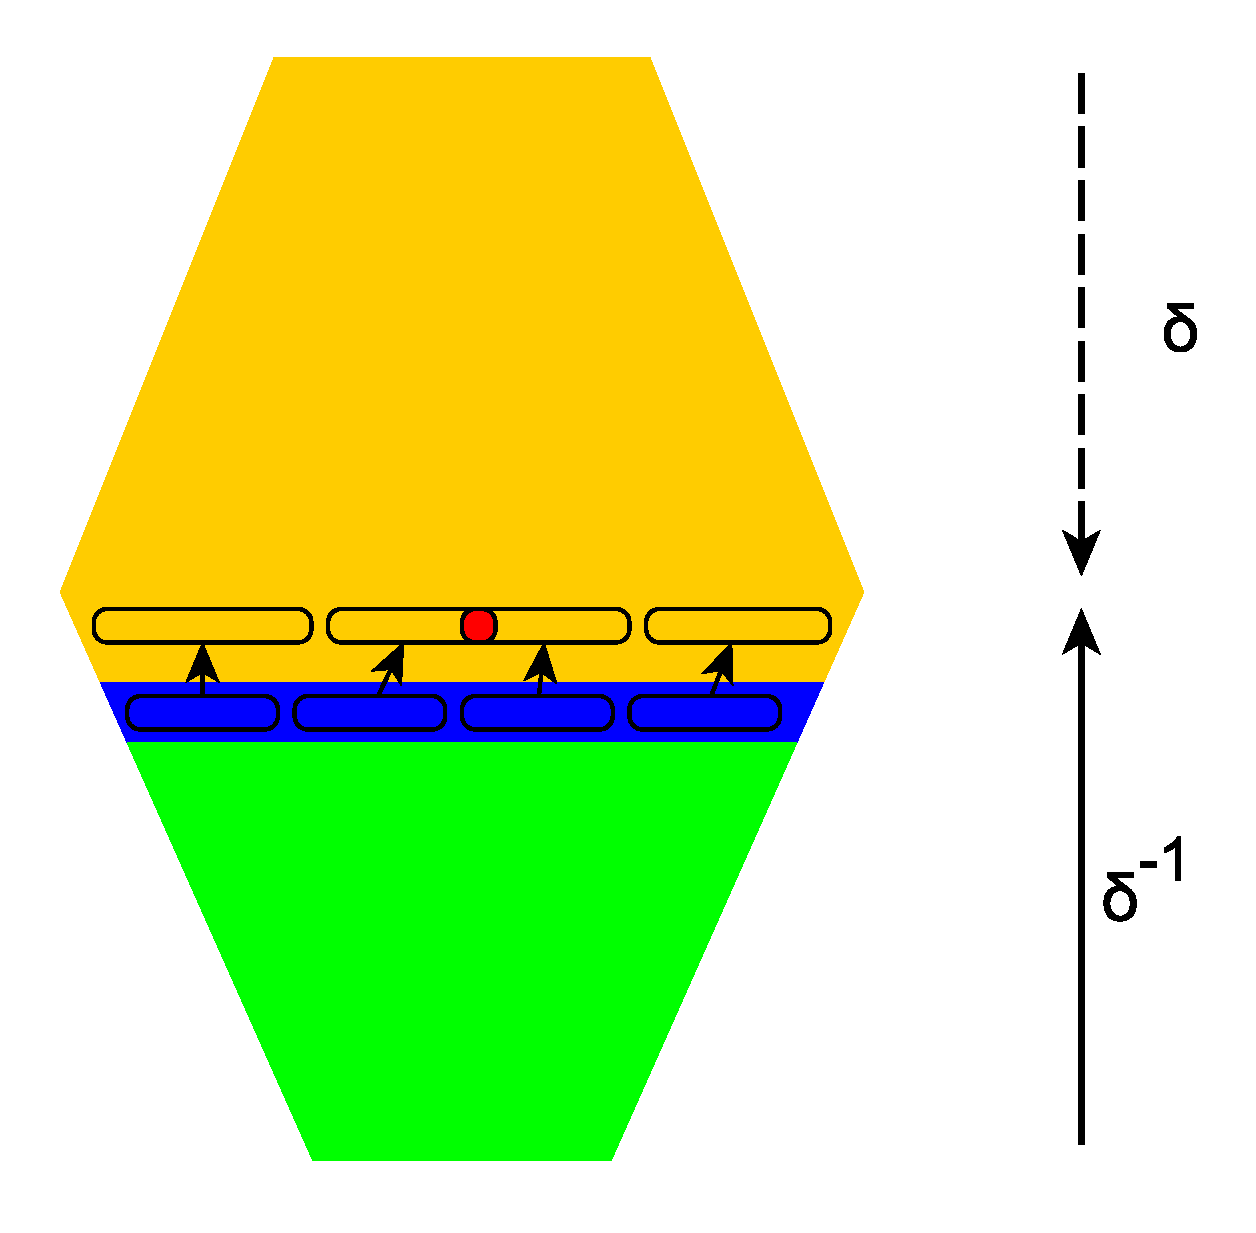
\includegraphics[height=0.8\textheight]{figs/f2r_parallel.pdf}
		%\caption{}
	\end{figure}
\end{frame}
%
%\begin{frame}{Parallelization of the First Phase}
%\small
%\begin{algorithm}[H]
%	\caption{BFS\_step\_F2R (in parallel)}
%	\label{algo:BFS-step-F2R-Parallel}
%	
%	\SetKwInOut{Input}{input}\SetKwInOut{Output}{output}
%	\Input{An automaton ${\cal A}=(S,\Sigma,\delta)$, the frontier $F$, the remaining set $R$, $\tau$}
%	\Output{The new frontier $F'$ and updated function $\tau$}
%	
%	\lForEach{thread $t$}{
%		$F'_t \longleftarrow \emptyset$
%	}
%	\ForEachP{$\{ s_i,s_j\} \in F$}
%	{
%		\ForEach{$x \in \Sigma$}
%		{
%			\ForEach{$\{ s'_i,s'_j\}$ where $s'_i \in \delta^{-1}(s_i,x)$ and $s'_j \in \delta^{-1}(s_j,x)$}
%			{
%				\If(\tcp*[h]{$\{ s'_i,s'_j\} \in R$}){$\tau({\{ s'_i,s'_j \}})$ is undefined}
%				{
%					$\tau(\{ s'_i,s'_j\}) \longleftarrow x \tau(\{ s_i,s_j \})$\;
%					$F'_t = F'_t \cup \{ \{ s'_i,s'_j \}  \} $\;
%				}
%			}
%		}
%	}
%	$F' \longleftarrow \emptyset$\;
%	\lForEach{thread t}{
%		$F' = F' \cup F'_t$
%	}
%\end{algorithm}
%\end{frame}

\subsection{Remaining to Frontier}

\begin{frame}{Another approach for PMF construction}
Can we apply BFS algorithm in a different way?

Use $\delta$ instead of $\delta^{-1}$: \alert{Remaining to Frontier}.
\end{frame}


\begin{frame}{Remaining to Frontier}
	\begin{figure}
		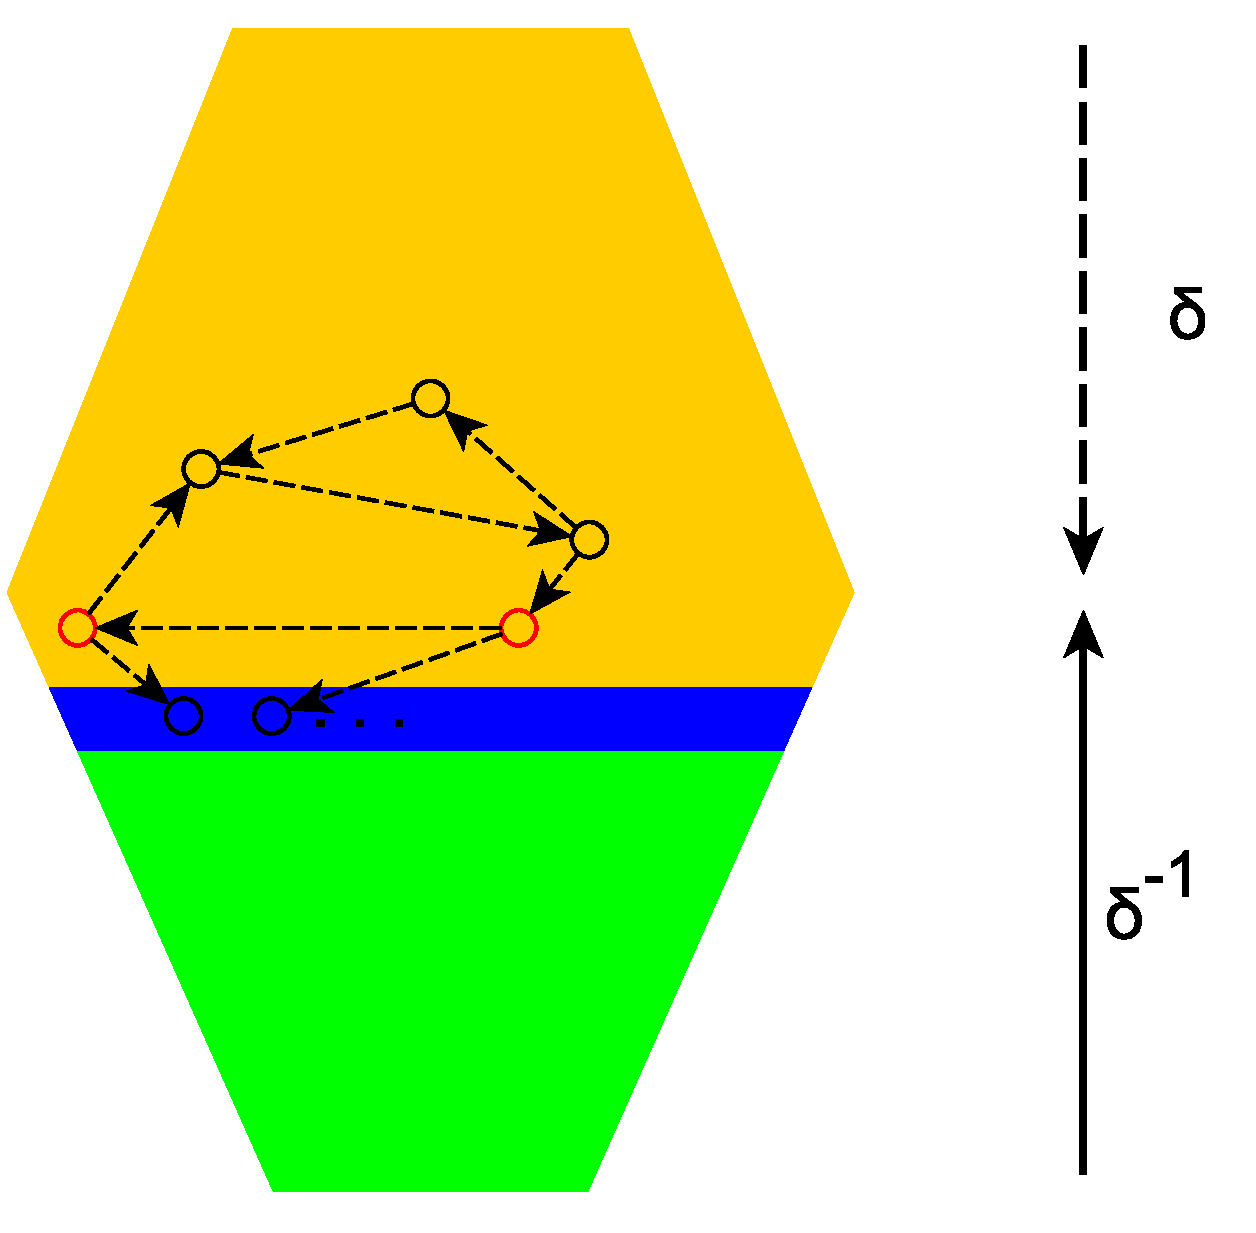
\includegraphics[height=0.8\textheight]{figs/r2f.pdf}
		%\caption{}
	\end{figure}
\end{frame}


\begin{frame}{Remaining to Frontier (in Parallel)}
	\begin{figure}
		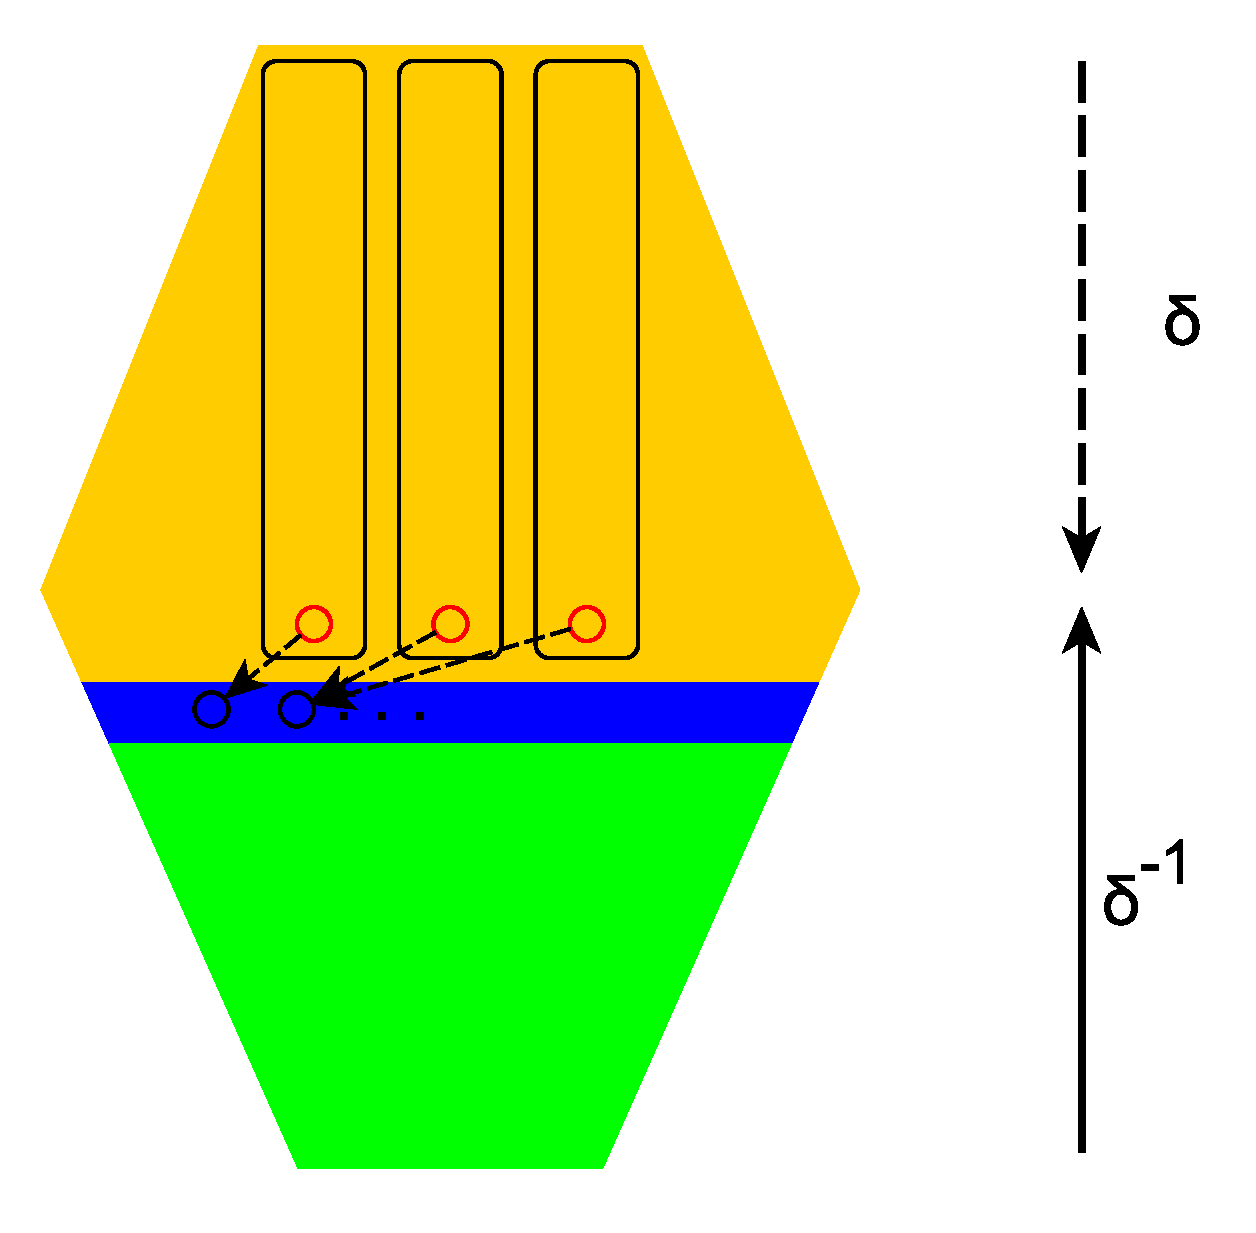
\includegraphics[height=0.8\textheight]{figs/r2f_parallel.pdf}
		%\caption{}
	\end{figure}
\end{frame}
%
%\begin{frame}{Remaining to Frontier}
%\footnotesize
%\begin{algorithm}[H]
%	\caption{BFS\_step\_R2F (in parallel)}
%	\label{algo:BFS-step-R2F-Parallel}
%	
%	\SetKwInOut{Input}{input}\SetKwInOut{Output}{output}
%	\Input{An automaton ${\cal A}=(S,\Sigma,\delta)$, the frontier $F$, the remaining set $R$, $\tau$}
%	\Output{The new frontier $F'$, the new remaining set $R'$, and updated function $\tau$}
%	
%		\lForEach{thread t}{$R'_t \longleftarrow \emptyset$}
%		\ForEachP{$\{ s_i,s_j \} \in R$}
%		{
%			$connected  \longleftarrow $ {\bf false}\;
%			\ForEach{$x \in \Sigma$}
%			{
%				$\{ s'_i, s'_j \}\longleftarrow \{ \delta(s_i,x),\delta(s_j,x) \}$; \\ 
%
%				\If(\tcp*[h]{$\{ s'_i,s'_j\} \in F$}){$\tau(\{ s'_i, s'_j \})$ is defined}
%				{
%					$\tau( \{ s_i, s_j\}) \longleftarrow x \tau(\{ s'_i, s'_j \})$\;
%					$connected  \longleftarrow $ {\bf true}\;
%					{\bf break}\;
%				}
%			}
%			\If{not $connected$}
%			{
%					$R'_t = R'_t \cup \{ \{ s_i, s_j \} \} $\;
%			}
%		}
%		$R' \longleftarrow \emptyset$\;
%		\lForEach{thread t}{
%			$R' = R' \cup R'_t$
%		}
%\end{algorithm}
%\end{frame}

\subsection{Hybrid Algorithm}
\begin{frame}{Comparison of R2F and F2R}
\begin{figure}[H]
	\centering
	\subfigure[$p = 8$, \# of vertices]{
		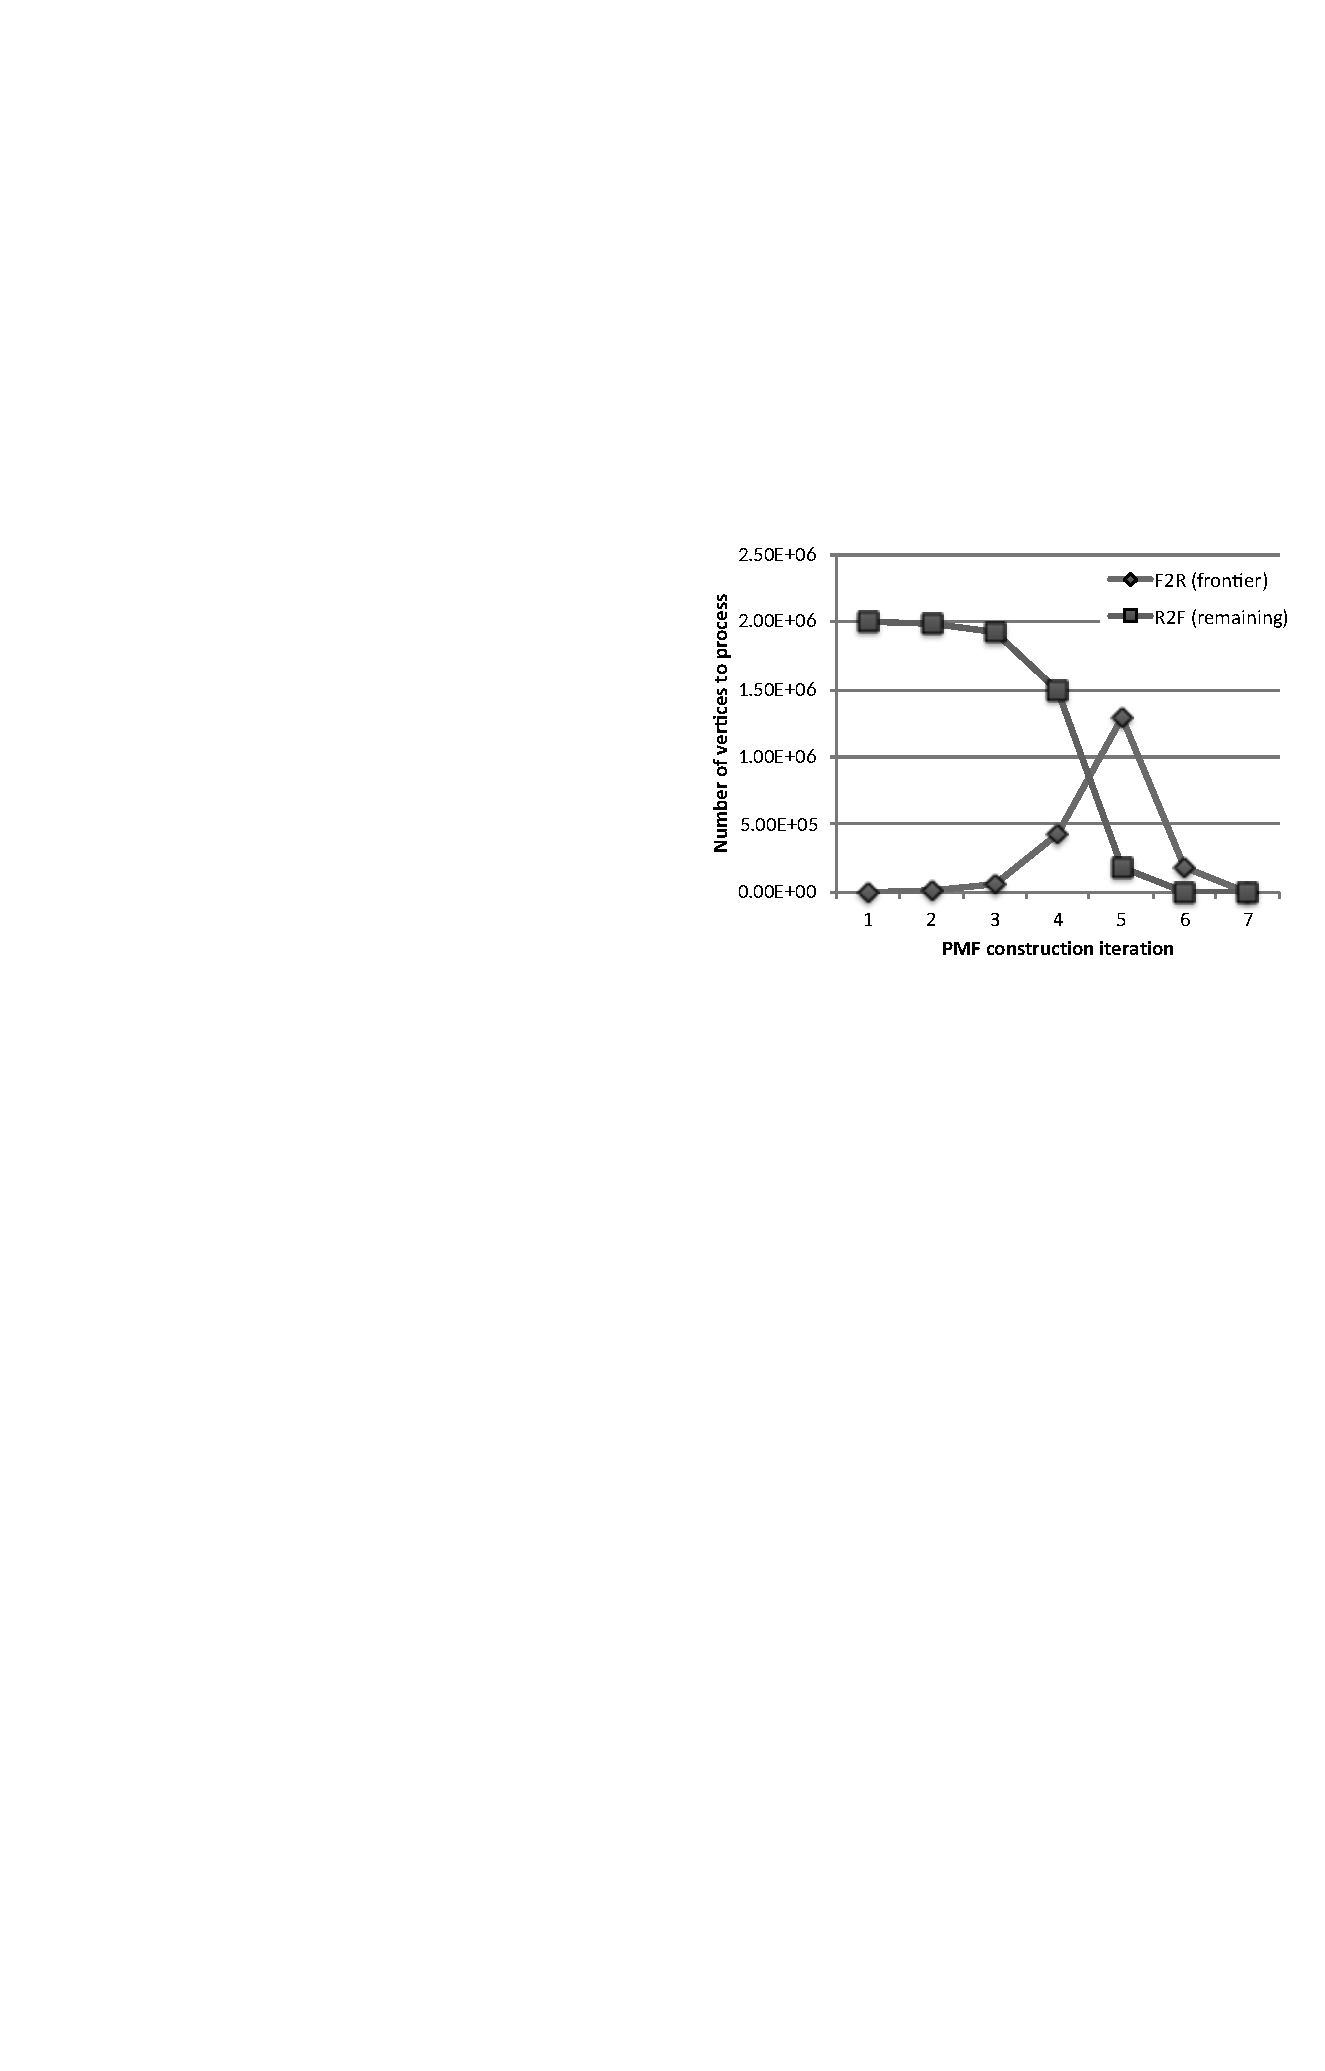
\includegraphics[height=0.5\textheight]{figs/8v_gray.pdf}
	}
	\subfigure[$p = 8$, execution time]{
		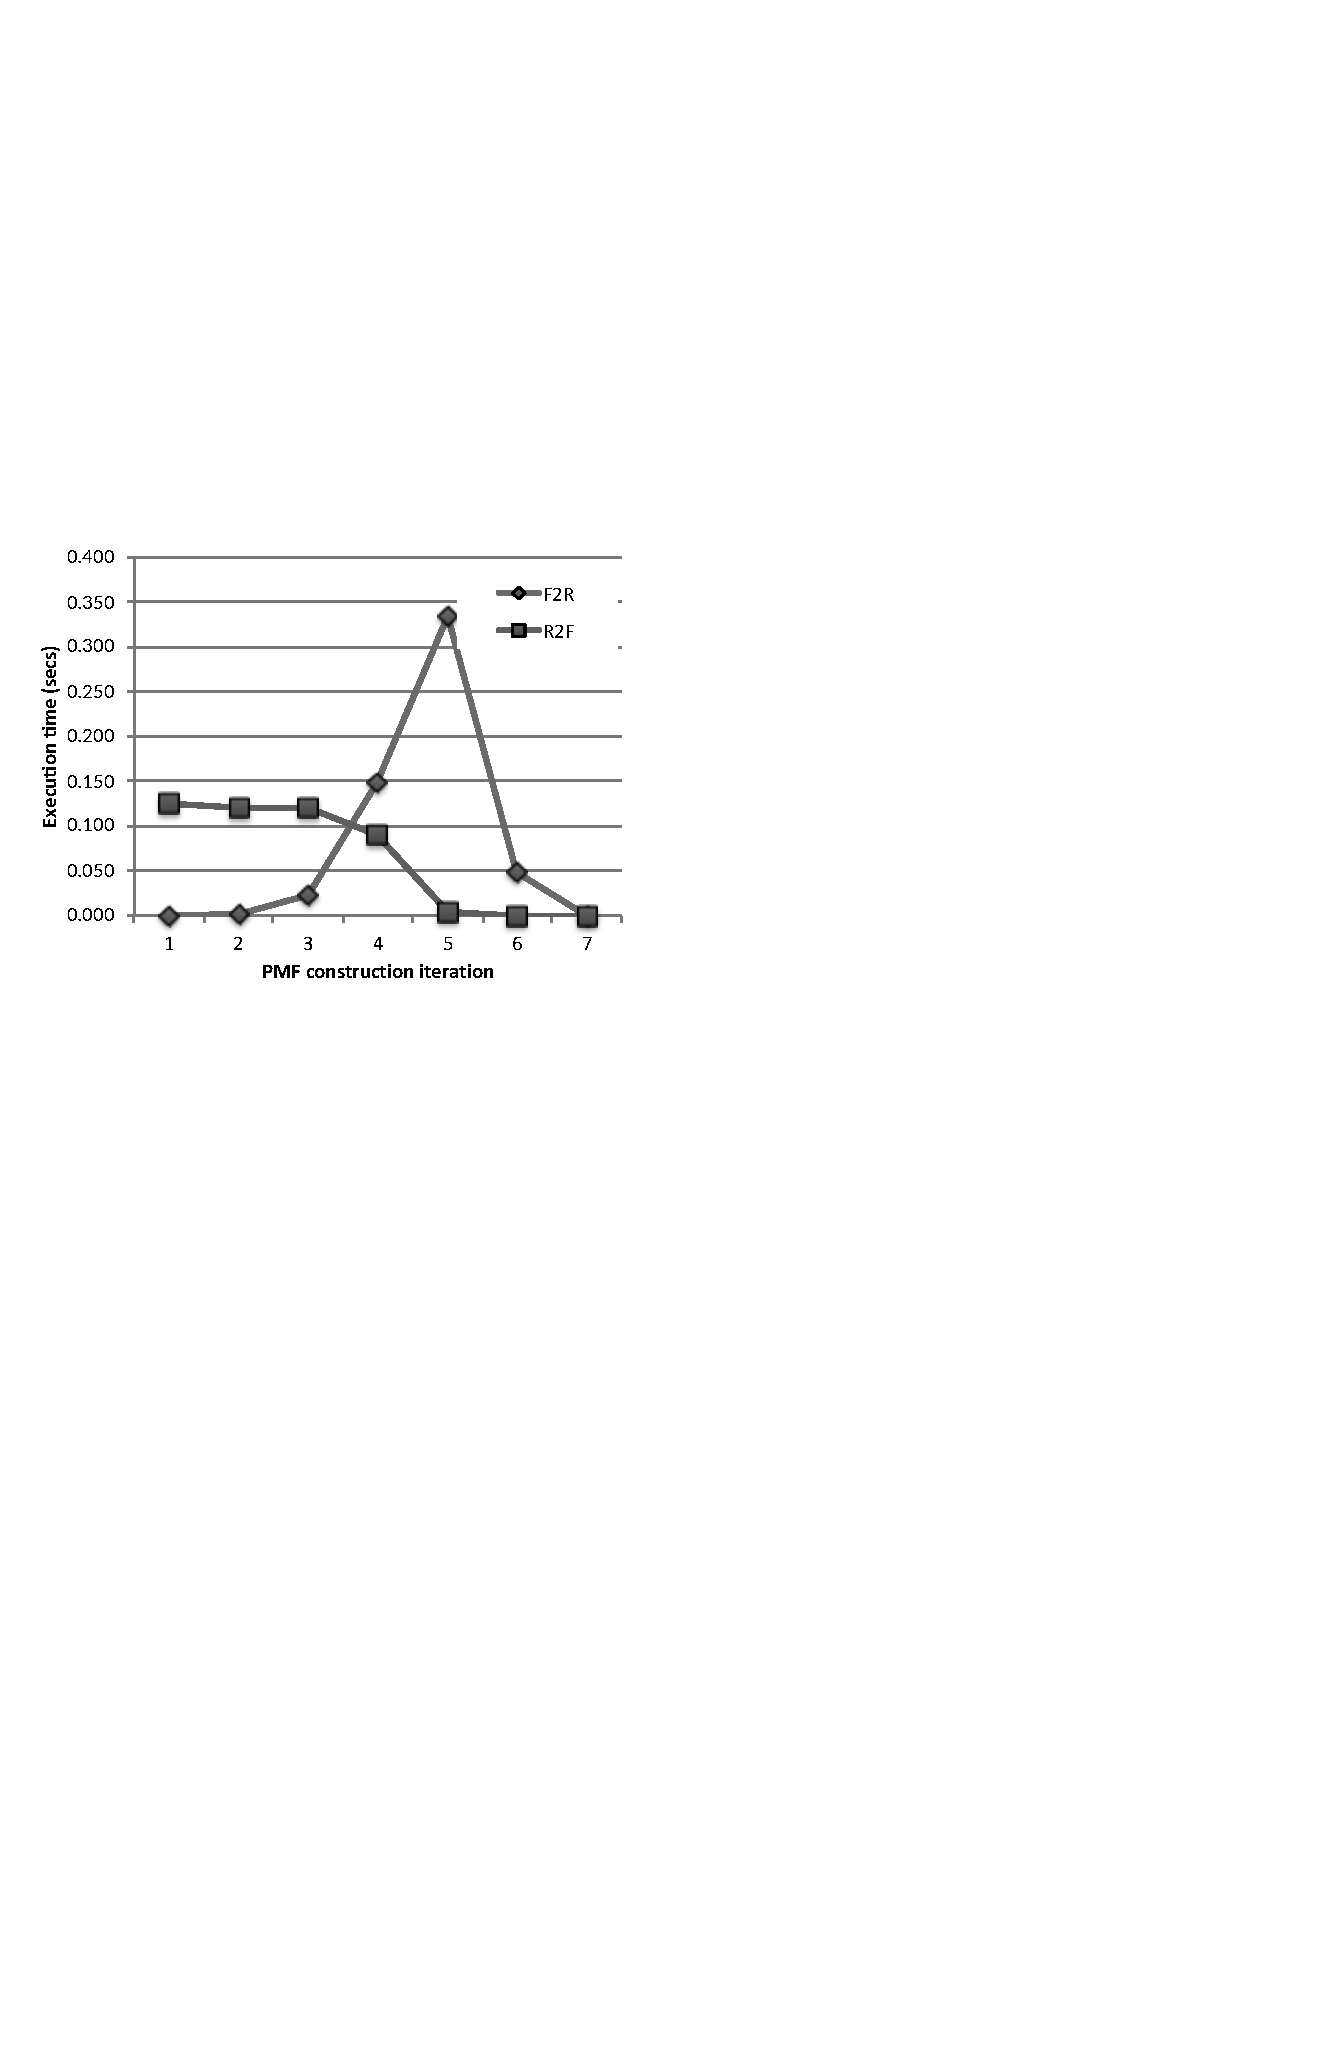
\includegraphics[height=0.5\textheight]{figs/8t_gray.pdf}
	}
	\caption{The number of frontier and remaining vertices at each BFS level and the corresponding execution times of F2R and R2F while constructing the PMF $\tau$ for $n = 2000$ and $p = 8$~(top) and $p=128$~(bottom).}
	
	\label{fig:BFS-vtcomparison}
\end{figure}
\end{frame}

\begin{frame}{Hybrid Algorithm}
\begin{algorithm}[H]
	\label{algo:BFS-Hybrid}
	\caption{Computing a function $\tau : S^{\langle 2 \rangle} \rightarrow \Sigma^\star$ (Hybrid)}
	
	\SetKwInOut{Input}{input}\SetKwInOut{Output}{output}
	\Input{An automaton ${\cal A}=(S,\Sigma,\delta)$}
	\Output{A function $\tau : S^{\langle 2 \rangle} \rightarrow \Sigma^\star$}
	

	\lForEach{singleton $\{ s,s \} \in S^{\langle 2 \rangle}$}{$\tau(\{ s,s \}) = \varepsilon$}
	\lForEach{pair $\{ s_i,s_j \} \in S^{\langle 2 \rangle}$}{$\tau(\{s_i,s_j\}) =${\em undefined}}
	
	$F \longleftarrow \{ \{ s,s \} | s \in S \}$\;
	$R \longleftarrow \{ \{ s_i,s_j \} | s_i,s_j \in S \wedge s_i \neq s_j \}$\;
	\While{$F$ is not empty}
	{
		\If{$|F| < |R|$}
		{
			$F,R,\tau \longleftarrow \mbox{BFS\_step\_F2R}(A,F,R,\tau)$\;
		}
		\Else
		{
			$F,R,\tau \longleftarrow \mbox{BFS\_step\_R2F}(A,F,R,\tau)$\;
		}
	}
\end{algorithm}
\end{frame}

\subsection{GPU Parallelization}
\begin{frame}{GPU Parallelization}
	Global synchronization is costly.
	
	\medskip
	
	Searching entire set of pairs instead of $F$ and $R$.
	
	\medskip
	
	Each thread checks one pair in the set.
\end{frame}

\begin{frame}{Indexing Mechanism}
	\begin{figure}
	\centering
	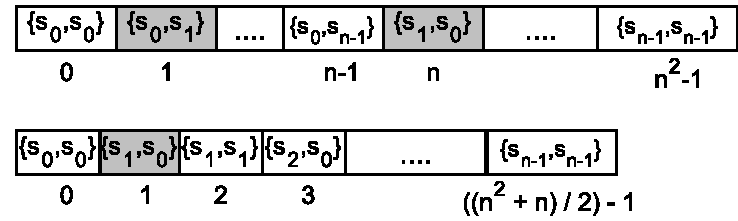
\includegraphics[width=\textwidth]{figs/memory.pdf}
	\caption{Indexing and placement of the state pair arrays. A simple placement of the pairs (on the left) uses redundant places for state pairs $\{s_i, s_j\}$, $i \neq j$, e.g., $\{s_1, s_2\}$ and $\{s_2, s_1\}$ in the figure. On the right, the indexing mechanism we used is shown.}
	\label{fig:mem}
\end{figure}
\end{frame}

\subsection{Parallelization of the Second Phase}
\begin{frame}{The Second Phase}
	Two sub-phases:
	\begin{itemize}
		\item Finding a pair with the minimum length of merging sequence among all active pairs
		\item Applying the merging sequence and finding the new active set
	\end{itemize}
	
	The execution time is negligible except for slowly synchronizing automata.
\end{frame}

\begin{frame}{Analysis on the Second Phase}
\begin{table}[ht]
	\begin{tabular}{r|rrr}
			
		n & $t_{FIND\_MIN}$ & $t_{SECOND\_PHASE}$ & $\frac{t_{FIND\_MIN}}{t_{SECOND\_PHASE}}$ \\\hline
		2000 & 4.729 & 4.741 & 0.997 \\
		4000 & 41.034 & 41.098 & 0.998 \\
		8000 & 1035.093 & 1035.48 & 1.000 \\
	\end{tabular}
	
	\caption{Comparison of the run time of the first sub-phase ($t_{FIND\_MIN}$), and the second phase ($t_{SECOND\_PHASE}$).}
	\label{table:phase-2-comparison}
\end{table}
\end{frame}

\begin{frame}{The Second Phase Parallelization}

	The first sub-phase is simply a finding minimum value from an array
	
	\medskip
	
	Parallelization is also simple:
	\begin{itemize}
		\item Elements of the array are  split among threads.
		\item Each thread finds the minimum locally.
		\item A thread finds the global minimum from local minimum values. 
	\end{itemize}
	
	\medskip
	
	Sorting the set of current states by their state numbers gives better spatial locality. 
\end{frame}

\section{Speeding Up the Fastest}
\begin{frame}{Can we speed up \textsc{Greedy} with single thread?}
\begin{table}[ht]
	\center
	\scalebox{0.7}{
	\begin{tabular}{r|rrr|rrr|rrr}
 		& \multicolumn{3}{c|}{n=2000} & \multicolumn{3}{c|}{n=4000} & \multicolumn{3}{c}{n=8000} \\
		p &  $h_{PMF}$ &  $h_{max}$ &  $h_{mean}$ &  $h_{PMF}$ &  $h_{max}$ &  $h_{mean}$ &  $h_{PMF}$ &  $h_{max}$ &  $h_{mean}$ \\ \hline
 		2 &  \textbf{14.2} &  \alert{10.0} &  1.9 &  \textbf{15.5} &  \alert{11.2} &  1.9 &  \textbf{16.9} &  \alert{12.1} &  1.9 \\
 		8 &  \textbf{5.0} &  \alert{4.0} &  1.3 &  \textbf{6.0} &  \alert{4.2} &  1.3 &  \textbf{6.0} &  \alert{4.6} &  1.3 \\
		32 &  \textbf{3.1} &  \alert{2.7} &  1.1 &  \textbf{4.0} &  \alert{2.9} &  1.1 &  \textbf{4.0} &  \alert{3.0} &  1.1 \\
		128 &  \textbf{3.0} &  \alert{2.0} &  1.0 &  \textbf{3.0} &  \alert{2.0} &  1.0 &  \textbf{3.0} &  \alert{2.1} &  1.0 \\
%		\v{C}ern\'y & 1999000.0 & 1952000.0 & 8884.8 & 7998000.0 & 7808000.0 & 19750.8 & 31996000.0 & 31232000.0 & 43480.8
	\end{tabular}}
	\caption{The length of longest merging sequence in PMF($h_{PMF}$) constructed in the first phase for random automata; maximum ($h_{max}$), and average ($h_{mean}$) lengths for merging sequences, used in the second phase of \textsc{Greedy}.}
\end{table}
\end{frame}

\subsection{Lazy Computation}
\begin{frame}{Lazy Computation}
	\begin{figure}
		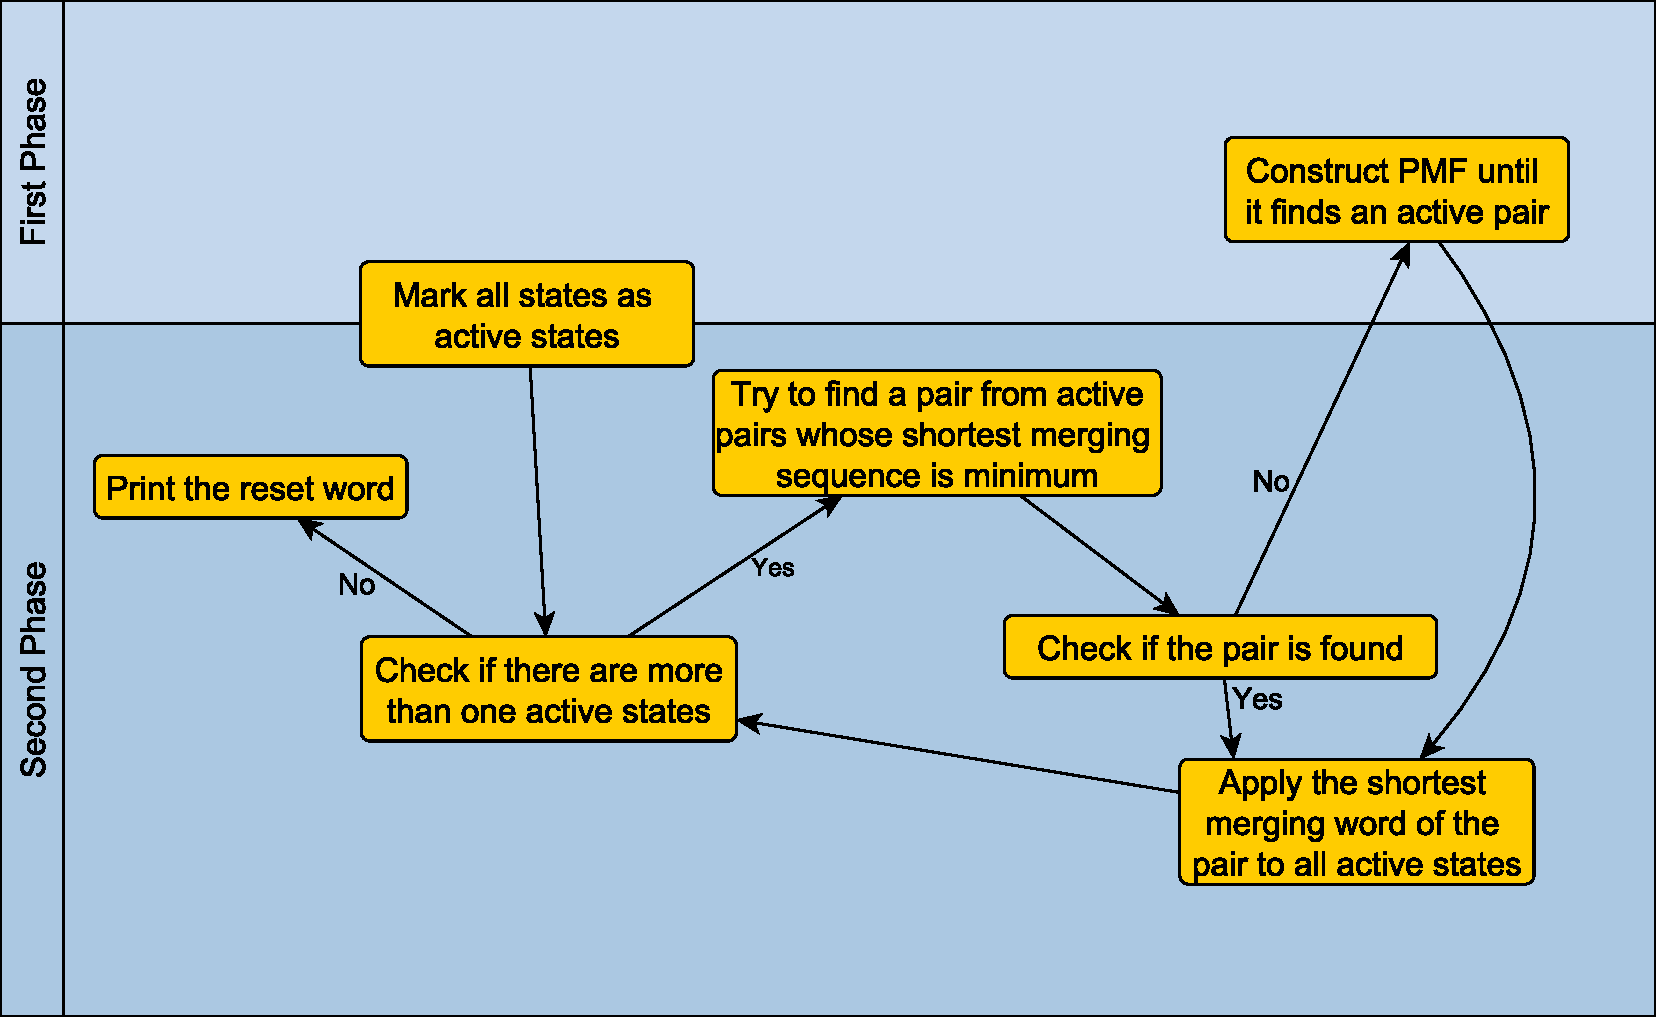
\includegraphics[width=\textwidth]{figs/lazy_flow.pdf}
	\end{figure}
\end{frame}


\begin{frame}{Can we make the algorithm Faster?}
\begin{table}[ht]
	\center
	\scalebox{0.7}{
	\begin{tabular}{r|rrr|rrr|rrr}
 		& \multicolumn{3}{c|}{n=2000} & \multicolumn{3}{c|}{n=4000} & \multicolumn{3}{c}{n=8000} \\
		p &  $h_{PMF}$ &  $h_{max}$ &  $h_{mean}$ &  $h_{PMF}$ &  $h_{max}$ &  $h_{mean}$ &  $h_{PMF}$ &  $h_{max}$ &  $h_{mean}$ \\ \hline
 		2 &  14.2 &  10.0 &  \alert{1.9} &  15.5 &  11.2 &  \alert{1.9} &  16.9 &  12.1 &  \alert{1.9} \\
 		8 &  5.0 &  4.0 &  \alert{1.3} &  6.0 &  4.2 &  \alert{1.3} &  6.0 &  4.6 &  \alert{1.3} \\
		32 &  3.1 &  2.7 &  \alert{1.1} &  4.0 &  2.9 &  \alert{1.1} &  4.0 &  3.0 &  \alert{1.1} \\
		128 &  3.0 &  2.0 &  \alert{1.0} &  3.0 &  2.0 &  \alert{1.0} &  3.0 &  2.1 &  \alert{1.0} \\
%		\v{C}ern\'y & 1999000.0 & 1952000.0 & 8884.8 & 7998000.0 & 7808000.0 & 19750.8 & 31996000.0 & 31232000.0 & 43480.8
	\end{tabular}}
	\caption{The length of longest merging sequence in PMF($h_{PMF}$) constructed in the first phase for random automata; maximum ($h_{max}$), and average ($h_{mean}$) lengths for merging sequences, used in the second phase of \textsc{Greedy}.}
\end{table}
\end{frame}


\subsection{Looking Ahead From the Current Pair}
\begin{frame}{Looking Ahead from the Current Pair}
\begin{figure}[ht]
	\centering
	\scalebox{0.75}{
		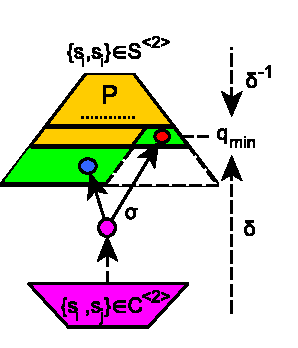
\includegraphics{figs/la.pdf}
	}
	\caption{The figure summarizes the lookahead process: The BFS forest~(the top part of the figure) is being constructed via $\delta^{-1}$ in a lazy way. However, $P = \{ \{s_i, s_j \} | \tau(\{s_i, s_j \})~ \mbox{\em is defined} \}$ and $C^{\langle 2 \rangle}$ are disconnected. The process tries to find a shortest path from $C^{\langle 2 \rangle}$ to the queue $Q$~(the green colored BFS frontier).}
	\label{fig:lookahead}
\end{figure}
\end{frame}


\begin{frame}{Looking Ahead from the Current Pair}
Applying lookahead process fully and every time is costly
\begin{itemize}
	\item \textsc{MaxStates}: Upper bound to decide when lookahead is used. $=log\ n$
	\item \textsc{MaxPairs}: Upper bound to decide when lookahead is done. $=n$
\end{itemize} 
\end{frame}


\subsection{Smart Way to Find Intersection of PMF and the Current Set}
\begin{frame}{Smart Way to Find Intersection of PMF and the Current Set}

\textbf{Naive Implementation:} Traverse the set of current pairs

\medskip

\textbf{Improvement:} Traverse the constructed PMF at early iterations. Traverse the set of current pairs later iterations.
\end{frame}

\section{Results}

\begin{frame}{Results}

\begin{figure}[ht]
	\centering
	\subfigure[$n = 2000$]{
		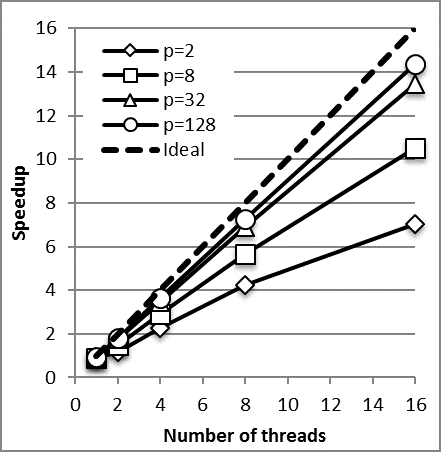
\includegraphics[height=0.42\textheight]{figs/spF2R_2000.png}
	}
	\subfigure[$n = 4000$]{
		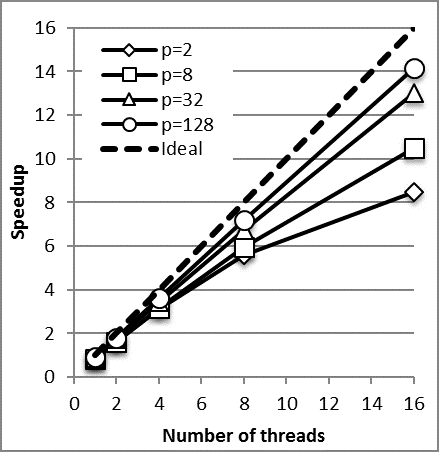
\includegraphics[height=0.42\textheight]{figs/spF2R_4000.png}
	}
	\subfigure[$n = 8000$]{
		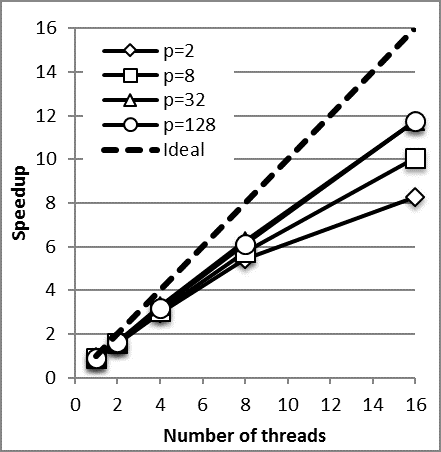
\includegraphics[height=0.42\textheight]{figs/spF2R_8000.png}
	}
	\caption{Speedups obtained with parallel F2R over the sequential PMF construction baseline.}
\end{figure}
\end{frame}

\begin{frame}{Results}
\begin{figure}[ht]
	\centering
	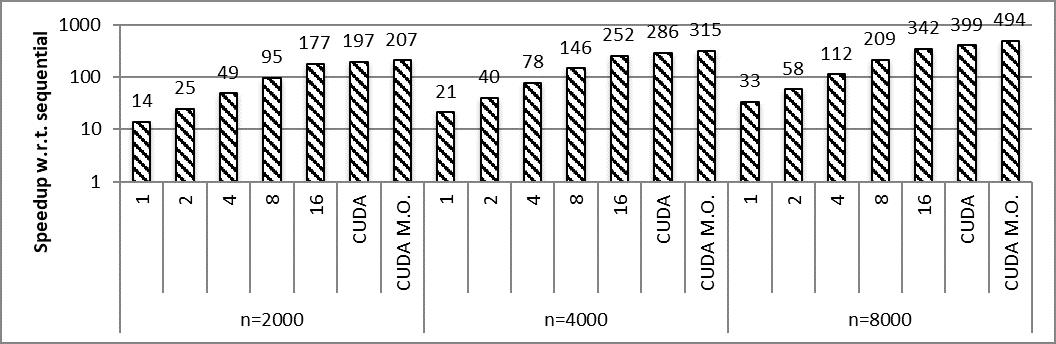
\includegraphics[height=0.4\textheight]{figs/hybrid_speedup_p128.png}
	
	\caption{The speedups of the Hybrid PMF construction algorithms with $p = 128$ and $n \in \{2000, 4000, 8000\}$. The $x$-axis shows the number of threads used for the Hybrid execution.  The values are computed based on the average sequential PMF construction time over $100$ different automata for each $(n, p)$ pair.}
	\label{fig:hybrid-speedup}
\end{figure}
\end{frame}

\begin{frame}{Results}
\begin{table}[ht]
	\center
	\scalebox{0.7}{
	\begin{tabular}{rr|rrr}
		& n & 2000 & 4000 & 8000\\\hline
		\multirow{2}{*}{sequential} & unsorted & 4.729 & 41.034 & 1035.093\\
		& sorted & 1.604 & 12.701 & 109.758\\\hline
		\multirow{2}{*}{1} & unsorted & 5.098 & 47.021 & 896.384\\
		& sorted & 2.553 & 20.274 & 168.116\\\hline
		\multirow{2}{*}{2} & unsorted & 3.869 & 37.352 & 874.253\\
		& sorted & 1.935 & 15.085 & 132.770\\\hline
		\multirow{2}{*}{4} & unsorted & 2.308 & 22.705 & 522.930\\
		& sorted & 1.178 & 8.946 & 75.673\\\hline
		\multirow{2}{*}{8} & unsorted & 1.259 & 13.131 & 289.750\\
		& sorted & 0.719 & 5.044 & 40.842\\\hline
		\multirow{2}{*}{16} & unsorted & 0.694 & 6.674 & 154.796\\
		& sorted & 0.723 & 3.350 & 22.403\\\hline
		\multirow{2}{*}{CUDA} & unsorted & 0.684 & 5.514 & 51.280\\
		& sorted & 0.391 & 1.556 & 9.613
	\end{tabular}}
	\caption{The execution times~(in seconds) of  the first sub-phase of the second phase.}
	\label{table:phase-2-time}
\end{table}
\end{frame}

\begin{frame}{Results}
\begin{table}[ht]
	\center
	\small
	\begin{tabular}{rr||r||rrr}
$n$		&	$p$	& Naive 	& Lazy		& Lookahaed & Smart \\\hline\hline
2000	& 2		& 99.99\%					& 40.31\%	& 1.71\%	& 1.71\%\\
		& 8		& 84.83\%					& 12.18\%	& 0.56\%	& 0.57\%\\
		& 32	& 37.41\%					& 3.64\%	& 0.25\%	& 0.25\%\\
		& 128	& 11.19\%					& 1.00\%	& 0.11\%	& 0.09\%\\\hline
4000	& 2		& 99.99\%					& 36.92\%	& 1.42\%	& 1.52\%\\
		& 8		& 87.11\%					& 11.72\%	& 0.42\%	& 0.45\%\\
		& 32	& 40.12\%					& 2.93\%	& 0.16\%	& 0.17\%\\
		& 128	& 12.08\%					& 0.94\%	& 0.07\%	& 0.08\%\\\hline
8000	& 2		& 100.00\%					& 37.56\%	& 1.31\%	& 1.24\%\\
		& 8		& 89.16\%					& 12.09\%	& 0.38\%	& 0.33\%\\
		& 32	& 42.78\%					& 3.08\%	& 0.11\%	& 0.06\%\\
		& 128	& 13.02\%					& 0.83\%	& 0.06\%	& 0.05\%
	\end{tabular}
	\caption{The percentage of processed edges}
	\label{table:edge-percent}
\end{table}
\end{frame}

\begin{frame}{Results}

\begin{figure}[ht]
	\centering
	\subfigure[$p = 32$]{
		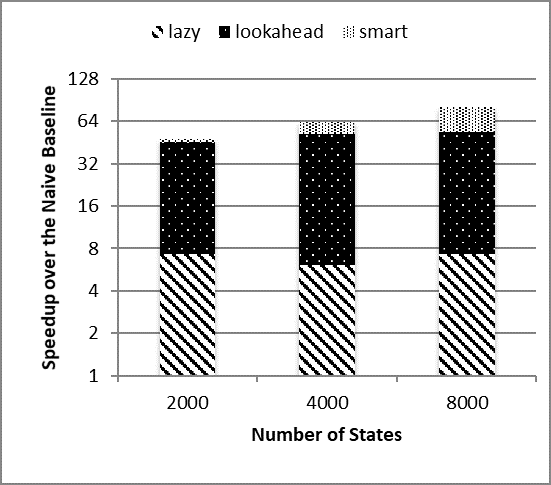
\includegraphics[width=0.45\textwidth]{figs/p32_greedy.png}
	}
	\subfigure[$p = 128$]{
		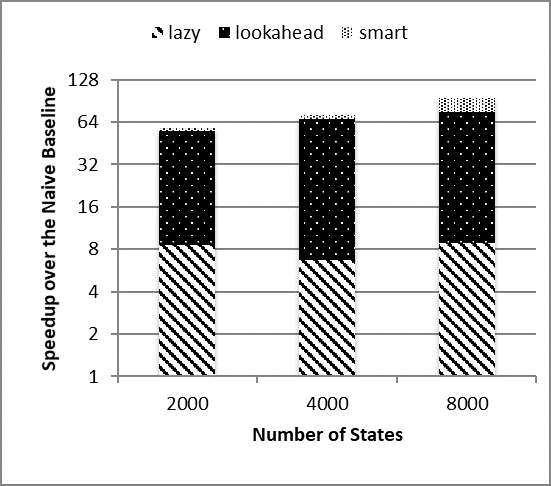
\includegraphics[width=0.45\textwidth]{figs/p128_greedy.png}
	}
	\caption{The speedup values normalized w.r.t. the naive baseline. For each additional improvement, the cumulative speedup is given with stacked columns.}
	\label{fig:speedups}
\end{figure}
\end{frame}

\section{Conclusion}

\begin{frame}{Conclusion}
\textsc{Greedy} is one of the fastest heuristics in literature.

\medskip

We speed up \textsc{Greedy} to make it more competitive:

\begin{itemize}
	\item First phase parallelization: up to $\times 500$ speed up
	\item Algorithmic optimization: up to $\times 100$ speed up
\end{itemize}

\end{frame}

\begin{frame}{Publications}
\small
Karahoda, S., Erenay, O. T., Kaya, K., T\"{u}rker, U. C., \& Yenig\"{u}n, H. (2016, October). Parallelizing Heuristics for Generating Synchronizing Sequences. In IFIP International Conference on Testing Software and Systems (pp. 106-122). Springer International Publishing.

\medskip

Karahoda, S., Kaya, K., \& Yenig\"{u}n, H. (2018). Synchronizing heuristics: Speeding up the fastest. Expert Systems with Applications, 94, 265-275.

\medskip

Altun, \"{O}. F., Atam, K. T., Karahoda, S., \& Kaya, K. (2017, October). Synchronizing Heuristics: Speeding up the Slowest. In IFIP International Conference on Testing Software and Systems (pp. 243-256). Springer, Cham.
Chicago	

\end{frame}

\begin{frame}{Acknowledgment}
This thesis was supported by The Scientific and Technological Research Council of Turkey (T\"{U}B\.{I}TAK) [grant number 114E569]. 
\end{frame}

\begin{frame}{}
\Huge
\center
Thank you for listening
\end{frame}
\end{document}
